\section{Algorithm}\label{section:algorithm}
In this section, we present the extended Raft algorithm, which is a variant of the Raft algorithm. It is designed for cluster with regular servers and at most one witness. The witness functions strictly as a follower server, implying that its role never transitions to candidate or leader. Furthermore, a witness only maintains a minimal set of metadata.

Our newly proposed algorithm minimizes data traffic and reduces the frequency of witness visits while preserving all key properties of the Raft algorithm. This implies that the extended Raft algorithm ensures that each of the following properties is consistently upheld. 

\begin{itemize}
    \item Election Safety
    \item Leader Append-only
    \item Log Matching
    \item Leader Completeness
    \item State Machine Safety
\end{itemize}

In the rest of this document, unless otherwise specified, the term 'server' will denote either a regular server or a witness. Consequently, the server set, denoted as $Server$, that constitutes a cluster could either be $RegularServer \cup {witness}$ or simply $RegularServer$, where $RegularServer$ is the set of all regular servers.


\subsection{Concepts and Definitions}\label{subsection:definition}

\begin{definition}
    A leader's \textbf{replication set} is a subset of the cluster server set, with its cardinality matching that of the regular server set.
\end{definition}

Let $ReplicationSets$ represent the set of all replication sets within a cluster. We have:
\begin{displaymath}
    ReplicationSets \defeq
    \begin{cases}
        \{Server\},                               & witness \notin Server \\
        \{Server \setminus \{x\}: x \in Server\}, & witness \in Server
    \end{cases}
\end{displaymath}

A leader maintains its replication set based on its view of the servers and modifies it under specific conditions. A leader may alter its replication set multiple times within a single term. To uniquely identify each replication set, we introduce the notion of a 'subterm' as detailed below.

\begin{definition} 
    A term is segmented into \textsc{subterms}, each begins with a replication set. 
\end{definition}

Subterms are sequentially numbered using consecutive integers, beginning from $0$ for each term. The leader retains its current subterm and increments it when the replication set is altered. Consequently, a leader's replication set remains static throughout its subterm.


\subsection{States}\label{subsection:states}

Figure \ref{fig:algo-state} illustrates the additional states introduced by the Extended Raft algorithm to accommodate the witness.
\begin{figure}[htbp]
    \begin{framed}
        \documentclass{standalone}

\usepackage{tlatex}
\usepackage{color}
\definecolor{boxshade}{gray}{.85}
\setboolean{shading}{true}

\usepackage{setspace}

\begin{document}
\onehalfspacing

    \begin{tla}

\* The following variables are used only on leaders:
\* The next entry to send to each follower.
VARIABLE nextIndex
\* The latest entry that each follower has acknowledged is the same as the
\* leader's. This is used to calculate commitIndex on the leader.
VARIABLE matchIndex
\* Leader's replication set
VARIABLE replicationSet
\* Leader's subterm number
VARIABLE currentSubterm
\* The latest subterm that this leader has written to the witness
VARIABLE witnessSubterm
leaderVars == <<nextIndex, matchIndex, elections, 
                replicationSet, currentSubterm, witnessSubterm>>

\* The following variables are persisted only on witness:
\* The latest replication set sent from leader
VARIABLE witnessReplicationSet
\* The latest term of replicated log entry
VARIABLE witnessLastLogTerm
\* The latest subterm of replicated log entry
VARIABLE witnessLastLogSubterm
witnessVars == <<witnessReplicationSet, 
                 witnessLastLogTerm, witnessLastLogSubterm>>

    \end{tla}
\begin{tlatex}
\@x{}%
\@y{%
  The following variables are used only on leaders:
}%
\@xx{}%
\@x{}%
\@y{%
  The next entry to send to each follower.
}%
\@xx{}%
\@x{ {\VARIABLE} nextIndex}%
\@x{}%
\@y{%
  The latest entry that each follower has acknowledged is the same as the
}%
\@xx{}%
\@x{}%
\@y{%
  leader's. This is used to calculate commitIndex on the leader.
}%
\@xx{}%
\@x{ {\VARIABLE} matchIndex}%
\@x{}%
\@y{%
  Leader's replication set
}%
\@xx{}%
\@x{ {\VARIABLE} replicationSet}%
\@x{}%
\@y{%
  Leader's subterm number
}%
\@xx{}%
\@x{ {\VARIABLE} currentSubterm}%
\@x{}%
\@y{%
  The latest subterm that this leader has written to the witness
}%
\@xx{}%
\@x{ {\VARIABLE} witnessSubterm}%
 \@x{ leaderVars \.{\defeq} {\langle} nextIndex ,\, matchIndex ,\, elections
 ,\,}%
 \@x{\@s{69.36} replicationSet ,\, currentSubterm ,\, witnessSubterm
 {\rangle}}%
\@pvspace{8.0pt}%
\@x{}%
\@y{%
  The following variables are persisted only on witness:
}%
\@xx{}%
\@x{}%
\@y{%
  The latest replication set sent from leader
}%
\@xx{}%
\@x{ {\VARIABLE} witnessReplicationSet}%
\@x{}%
\@y{%
  The latest term of replicated log entry
}%
\@xx{}%
\@x{ {\VARIABLE} witnessLastLogTerm}%
\@x{}%
\@y{%
  The latest subterm of replicated log entry
}%
\@xx{}%
\@x{ {\VARIABLE} witnessLastLogSubterm}%
\@x{ witnessVars \.{\defeq} {\langle} witnessReplicationSet ,\,}%
\@x{\@s{75.11} witnessLastLogTerm ,\, witnessLastLogSubterm {\rangle}}%
\@pvspace{8.0pt}%
\end{tlatex}
\end{document}


    \end{framed}
    \caption{State}
    \label{fig:algo-state}
\end{figure}

Each leader maintains three additional volatile variables: $replicationSet$, $currentSubterm$, and $witnessSubterm$. The $replicationSet$ represents the leader's current replication set, initialized to $RegularServer$, and is modified by $AdjustReplicationSet$ action. The $currentSubterm$ represents the latest subterm of the leader, initialized to $0$ and incremented upon a change in the leader's replication set. The $witnessSubterm$ denotes the latest subterm during which the leader replicated its log entry to the witness.

In addition to $currentTerm$ and $votedFor$, the witness also includes $witnessReplicationSet$, $witnessLastLogTerm$, and $witnessLastLogSubterm$. These represent the most recent replication set, log entry term, and log entry subterm that the leader sent to the witness. We will further discuss this in Section \ref{subsection:log-replication}.

Beyond the additional states in the leader and witness, each log entry is also associated with the leader's current subterm number when it is appended to the leader's log (Figure \ref{fig:client-request}). This subterm number is replicated and persisted alongside the log entry on all regular servers. We now denote a log entry as $\entry{index,term,subterm}$, which is uniquely identified by $index$ and $term$, and associated with $subterm$.

\begin{figure}
    \begin{framed}
        \documentclass[preview, border={5pt 0pt 5pt 1pt}]{standalone}

\usepackage{tlatex}
\usepackage{color}
\definecolor{boxshade}{gray}{.85}
\setboolean{shading}{true}

\usepackage{setspace}

\begin{document}
\onehalfspacing

    \begin{tla}

\* Leader i receives a client request to add v to the log.
ClientRequest(i, v) ==
    /\ state[i] = Leader
    /\ LET entry  == [term       |-> currentTerm[i],
                      subterm    |-> currentSubterm[i],
                      value      |-> v]
           newLog == Append(log[i], entry)
        IN log' = [log EXCEPT ![i] = newLog]
    /\ UNCHANGED <<messages, serverVars, candidateVars, 
                   leaderVars, commitIndex, witnessVars>>
        
    \end{tla}
\begin{tlatex}
\@x{}%
\@y{%
  Leader i receives a client request to add v to the log.
}%
\@xx{}%
\@x{ ClientRequest ( i ,\, v ) \.{\defeq}}%
\@x{\@s{16.4} \.{\land} state [ i ] \.{=} Leader}%
 \@x{\@s{16.4} \.{\land} \.{\LET} entry\@s{13.31} \.{\defeq} [ term\@s{26.35}
 \.{\mapsto} currentTerm [ i ] ,\,}%
\@x{\@s{106.38} subterm\@s{12.30} \.{\mapsto} currentSubterm [ i ] ,\,}%
\@x{\@s{106.38} value\@s{24.45} \.{\mapsto} v ]}%
\@x{\@s{52.01} newLog \.{\defeq} Append ( log [ i ] ,\, entry )}%
 \@x{\@s{31.61} \.{\IN} log \.{'} \.{=} [ log {\EXCEPT} {\bang} [ i ] \.{=}
 newLog ]}%
 \@x{\@s{16.4} \.{\land} {\UNCHANGED} {\langle} messages ,\, serverVars ,\,
 candidateVars ,\,}%
\@x{\@s{89.98} leaderVars ,\, commitIndex ,\, witnessVars {\rangle}}%
\@pvspace{8.0pt}%
\end{tlatex}

\end{document}




    \end{framed}
    \caption{Client request}
    \label{fig:client-request}
\end{figure}

\subsection{Log Replication} \label{subsection:log-replication}
The leader replicates its log to regular servers in the exact same way as that in the Raft algorithm, and the regular servers handle the received log entries in the same way as well.

However, for the witness, log replication is performed differently, as shown in Figure \ref{fig:algo-append-entries-to-witness}. In the Extended Raft algorithm, the leader sends an $AppendEntriesToWitnessRequest$ to the witness, which includes the current replication and metadata of the log entry that satisfies the following conditions:
\begin{enumerate} 
    \item\label{cond:in-subterm} The log entry's term and subterm are equal to $currentTerm$ and $currentSubterm$, respectively. 
    \item The leader's current replication set includes the witness. 
    \item The leader has received acknowledgments for the log entry from at least a subquorum (one server away from forming a quorum) in the leader's current replication set. 
    \item\label{condition:first-in-subterm} The leader has not received any acknowledgment from the witness during the current subterm. 
\end{enumerate}

\begin{figure}[htbp]
    \begin{framed}
        \documentclass{standalone}

\usepackage{tlatex}
\usepackage{color}
\definecolor{boxshade}{gray}{.85}
\setboolean{shading}{true}

\usepackage{setspace}

\begin{document}
\onehalfspacing

    \begin{tla}

\* Leader i sends witness an AppendEntriesToWitness request with log entry 
\* in current subterm acknowledged by a subquorum in current replication set.
AppendEntriesToWitness(i) ==
    /\ state[i] = Leader
    /\ WitnessID \in replicationSet[i]
    /\ LET Agree(index) == 
               {i} \cup {k \in replicationSet[i]: matchIndex[i][k] >= index}
           IsAgreed(k)  ==
               /\ log[i][k].term    = currentTerm[i]
               /\ log[i][k].subterm = currentSubterm[i]
               /\ ({WitnessID} \cup Agree(k)) \in Quorum
           agreeIndexes == { k \in 1..Len(log[i]): IsAgreed(k) }
           lastEntry    == Max(agreedIndex)
       IN /\ agreeIndexes /= {}
          /\ \/ \* witnessSubterm never exceeds currentSubterm following specification
                /\ currentSubterm[i] > witnessSubterm
                /\ Send([mtype           |-> AppendEntriesToWitnessRequest,
                         mterm           |-> currentTerm[i],
                         mlogTerm        |-> log[i][lastEntry].term,
                         mlogSubterm     |-> log[i][lastEntry].subterm,
                         mreplicationSet |-> replicaitonSet[i],
                         mindex          |-> lastEntry,
                         \* mlog and mentries are used as history variable for
                         \* the proof. They do not exist in a real implementation.
                         mlog            |-> log[i],
                         mentries        |-> SubSeq(log[i], 1, lastEntry),
                         msource         |-> i,
                         mdest           |-> WitnessID])
                /\ UNCHANGED <<leaderVars>>
             \/ \* shortcut replication
                /\ currentSubterm[i] = witnessSubterm[i]
                /\ Send([mtype           |-> AppendEntriesResponse,
                         mterm           |-> currentTerm[i],
                         msuccess        |-> TRUE,
                         mmatchIndex     |-> lastEntry,
                         msource         |-> WitnessID,
                         mdest           |-> i])
    /\ UNCHANGED <<serverVars, candidateVars, logVars, witnessVars>>
    \end{tla}
\begin{tlatex}
\@x{}%
\@y{%
  Leader i sends witness an AppendEntriesToWitness request with log entry 
}%
\@xx{}%
\@x{}%
\@y{%
  in current subterm acknowledged by a subquorum in current replication set.
}%
\@xx{}%
\@x{ AppendEntriesToWitness ( i ) \.{\defeq}}%
\@x{\@s{16.4} \.{\land} state [ i ] \.{=} Leader}%
\@x{\@s{16.4} \.{\land} WitnessID \.{\in} replicationSet [ i ]}%
\@x{\@s{16.4} \.{\land} \.{\LET} Agree ( index ) \.{\defeq}}%
 \@x{\@s{64.31} \{ i \} \.{\cup} \{ k \.{\in} replicationSet [ i ] \.{:}
 matchIndex [ i ] [ k ] \.{\geq} index \}}%
\@x{\@s{47.91} IsAgreed ( k )\@s{4.1} \.{\defeq}}%
 \@x{\@s{64.31} \.{\land} log [ i ] [ k ] . term\@s{14.05} \.{=} currentTerm [
 i ]}%
 \@x{\@s{64.31} \.{\land} log [ i ] [ k ] . subterm \.{=} currentSubterm [ i
 ]}%
 \@x{\@s{64.31} \.{\land} ( \{ WitnessID \} \.{\cup} Agree ( k ) ) \.{\in}
 Quorum}%
 \@x{\@s{47.91} agreeIndexes \.{\defeq} \{ k \.{\in} 1 \.{\dotdot} Len ( log [
 i ] ) \.{:} IsAgreed ( k ) \}}%
\@x{\@s{47.91} lastEntry\@s{14.68} \.{\defeq} Max ( agreedIndex )}%
\@x{\@s{27.51} \.{\IN} \.{\land} agreeIndexes \.{\neq} \{ \}}%
\@x{\@s{47.91} \.{\land} \.{\lor}}%
\@y{%
  witnessSubterm never exceeds currentSubterm following specification
}%
\@xx{}%
\@x{\@s{70.13} \.{\land} currentSubterm [ i ] \.{>} witnessSubterm}%
 \@x{\@s{70.13} \.{\land} Send ( [ mtype\@s{41.72} \.{\mapsto}
 AppendEntriesToWitnessRequest ,\,}%
\@x{\@s{109.89} mterm\@s{38.77} \.{\mapsto} currentTerm [ i ] ,\,}%
 \@x{\@s{109.89} mlogTerm\@s{23.94} \.{\mapsto} log [ i ] [ lastEntry ] . term
 ,\,}%
 \@x{\@s{109.89} mlogSubterm\@s{11.42} \.{\mapsto} log [ i ] [ lastEntry ] .
 subterm ,\,}%
\@x{\@s{109.89} mreplicationSet \.{\mapsto} replicaitonSet [ i ] ,\,}%
\@x{\@s{109.89} mindex\@s{35.61} \.{\mapsto} lastEntry ,\,}%
\@x{\@s{109.89}}%
\@y{%
  mlog and mentries are used as history variable for
}%
\@xx{}%
\@x{\@s{109.89}}%
\@y{%
  the proof. They do not exist in a real implementation.
}%
\@xx{}%
\@x{\@s{109.89} mlog\@s{46.39} \.{\mapsto} log [ i ] ,\,}%
 \@x{\@s{109.89} mentries\@s{28.7} \.{\mapsto} SubSeq ( log [ i ] ,\, 1 ,\,
 lastEntry ) ,\,}%
\@x{\@s{109.89} msource\@s{32.8} \.{\mapsto} i ,\,}%
\@x{\@s{109.89} mdest\@s{40.96} \.{\mapsto} WitnessID ] )}%
\@x{\@s{70.13} \.{\land} {\UNCHANGED} {\langle} leaderVars {\rangle}}%
\@x{\@s{59.02} \.{\lor}}%
\@y{%
  shortcut replication
}%
\@xx{}%
\@x{\@s{70.13} \.{\land} currentSubterm [ i ] \.{=} witnessSubterm [ i ]}%
 \@x{\@s{70.13} \.{\land} Send ( [ mtype\@s{49.62} \.{\mapsto}
 AppendEntriesResponse ,\,}%
\@x{\@s{109.89} mterm\@s{46.67} \.{\mapsto} currentTerm [ i ] ,\,}%
\@x{\@s{109.89} msuccess\@s{36.52} \.{\mapsto} {\TRUE} ,\,}%
\@x{\@s{109.89} mmatchIndex\@s{16.4} \.{\mapsto} lastEntry ,\,}%
\@x{\@s{109.89} msource\@s{40.04} \.{\mapsto} WitnessID ,\,}%
\@x{\@s{109.89} mdest\@s{49.68} \.{\mapsto} i ] )}%
 \@x{\@s{16.4} \.{\land} {\UNCHANGED} {\langle} serverVars ,\, candidateVars
 ,\, logVars ,\, witnessVars {\rangle}}%
\end{tlatex}
\end{document}


    \end{framed}
    
    \caption{AppendEntriesToWitness}
    \label{fig:append-entries-to-witness}
\end{figure}

The $AppendEntriesToWitness$ can be considered as a special implementation of the $AppendEntries$ action with batching of log prefix up to a specific log entry. This log entry belongs to the current subterm and has received subquorum acknowledgements from the current replication set. In addition to the message fields that also exist in $AppendEntriesRequest$, the dispatched message $AppendEntriesToWitnessReques$ also contains the current replication set and the metadata of the last batched entries.

Upon receiving the request, the witness persists the replication set, as well as the term and subterm of the log entry, then responds to the leader with an $AppendEntriesResponse$ message (Figure \ref{fig:handle-append-entries-to-witness}). 

\begin{figure}
    \begin{framed}
        \documentclass{standalone}

\usepackage{tlatex}
\usepackage{color}
\definecolor{boxshade}{gray}{.85}
\setboolean{shading}{true}

\usepackage{setspace}

\begin{document}
\onehalfspacing

    \begin{tla}

\* Witness receives an AppendEntriesToWitnessRequest from server j with
\* m.mterm <= currentTerm[WitnessID]. 
HandleAppendEntriesToWitnessRequest(j, m) ==
    /\ m.mterm <= currentTerm[WitnessID]
    /\ \/ \* reject request
          /\ m.mterm < currentTerm[WitnessID]
          /\ Reply([mtype           |-> AppendEntriesResponse,
                    mterm           |-> currentTerm[WitnessID],
                    msuccess        |-> FALSE,
                    mmatchIndex     |-> 0,
                    msource         |-> WitnessID,
                    mdest           |-> j],
                    m)
          /\ UNCHANGED <<serverVars, logVars, witnessVars>>
       \/ \* accept request, always no conflict.
          /\ m.mterm = currentTerm[WitnessID]
          /\ \/ m.mlastLogTerm > witnessLastLogTerm[WitnessID]
             \/ /\ m.mlastLogTerm = witnessLastLogTerm[WitnessID]
                /\ m.mlastLogSubterm > witnessLastLogSubterm[WitnessID]
          /\ witnessReplicationSet' = 
              [witnessReplicationSet EXCEPT![WitnessID] = m.mreplicationSet]
          /\ witnessLastLogTerm' =
              [witnessLastLogTerm EXCEPT![WitnessID] = m.mlastLogTerm]
          /\ witnessLastLogSubterm' =
              [witnessLastLogSubterm EXCEPT![WitnessID] = m.mlastLogSubterm]
          \* log will not be modified in real implementation. It is only
          \* used here for the proof.
          /\ log' = [log EXCEPT![WitnessID] = m.mentries]
          /\ Reply([mtype           |-> AppendEntriesResponse,
                    mterm           |-> currentTerm[WitnessID],
                    msuccess        |-> TRUE,
                    mmatchIndex     |-> m.mindex,
                    msource         |-> WitnessID,
                    mdest           |-> j],
                    m)
          /\ UNCHANGED <<serverVars, log>>
    /\ UNCHANGED <<candidateVars, leaderVars>>
    \end{tla}
\begin{tlatex}
\@x{}%
\@y{%
  Witness receives an AppendEntriesToWitnessRequest from server j with
}%
\@xx{}%
\@x{}%
\@y{%
  m.mterm <= currentTerm[WitnessID]. 
}%
\@xx{}%
\@x{ HandleAppendEntriesToWitnessRequest ( j ,\, m ) \.{\defeq}}%
\@x{\@s{16.4} \.{\land} m . mterm \.{\leq} currentTerm [ WitnessID ]}%
\@x{\@s{16.4} \.{\land} \.{\lor}}%
\@y{%
  reject request
}%
\@xx{}%
\@x{\@s{38.62} \.{\land} m . mterm \.{<} currentTerm [ WitnessID ]}%
 \@x{\@s{38.62} \.{\land} Reply ( [ mtype\@s{49.62} \.{\mapsto}
 AppendEntriesResponse ,\,}%
\@x{\@s{81.18} mterm\@s{46.67} \.{\mapsto} currentTerm [ WitnessID ] ,\,}%
\@x{\@s{81.18} msuccess\@s{36.52} \.{\mapsto} {\FALSE} ,\,}%
\@x{\@s{81.18} mmatchIndex\@s{16.40} \.{\mapsto} 0 ,\,}%
\@x{\@s{81.18} msource\@s{40.04} \.{\mapsto} WitnessID ,\,}%
\@x{\@s{81.18} mdest\@s{49.68} \.{\mapsto} j ] ,\,}%
\@x{\@s{81.18} m )}%
 \@x{\@s{38.62} \.{\land} {\UNCHANGED} {\langle} serverVars ,\, logVars ,\,
 witnessVars {\rangle}}%
\@x{\@s{27.51} \.{\lor}}%
\@y{%
  accept request, always no conflict.
}%
\@xx{}%
\@x{\@s{38.62} \.{\land} m . mterm \.{=} currentTerm [ WitnessID ]}%
 \@x{\@s{38.62} \.{\land} \.{\lor} m . mlastLogTerm \.{>} witnessLastLogTerm [
 WitnessID ]}%
 \@x{\@s{49.73} \.{\lor} \.{\land} m . mlastLogTerm \.{=} witnessLastLogTerm [
 WitnessID ]}%
 \@x{\@s{60.84} \.{\land} m . mlastLogSubterm \.{>} witnessLastLogSubterm [
 WitnessID ]}%
\@x{\@s{38.62} \.{\land} witnessReplicationSet \.{'} \.{=}}%
 \@x{\@s{53.83} [ witnessReplicationSet {\EXCEPT} {\bang} [ WitnessID ] \.{=}
 m . mreplicationSet ]}%
\@x{\@s{38.62} \.{\land} witnessLastLogTerm \.{'} \.{=}}%
 \@x{\@s{53.83} [ witnessLastLogTerm {\EXCEPT} {\bang} [ WitnessID ] \.{=} m .
 mlastLogTerm ]}%
\@x{\@s{38.62} \.{\land} witnessLastLogSubterm \.{'} \.{=}}%
 \@x{\@s{53.83} [ witnessLastLogSubterm {\EXCEPT} {\bang} [ WitnessID ] \.{=}
 m . mlastLogSubterm ]}%
\@x{\@s{38.62}}%
\@y{%
  log will not be modified in real implementation. It is only
}%
\@xx{}%
\@x{\@s{38.62}}%
\@y{%
  used here for the proof.
}%
\@xx{}%
 \@x{\@s{38.62} \.{\land} log \.{'} \.{=} [ log {\EXCEPT} {\bang} [ WitnessID
 ] \.{=} m . mentries ]}%
 \@x{\@s{38.62} \.{\land} Reply ( [ mtype\@s{49.62} \.{\mapsto}
 AppendEntriesResponse ,\,}%
\@x{\@s{81.18} mterm\@s{46.67} \.{\mapsto} currentTerm [ WitnessID ] ,\,}%
\@x{\@s{81.18} msuccess\@s{36.52} \.{\mapsto} {\TRUE} ,\,}%
\@x{\@s{81.18} mmatchIndex\@s{16.40} \.{\mapsto} m . mindex ,\,}%
\@x{\@s{81.18} msource\@s{40.04} \.{\mapsto} WitnessID ,\,}%
\@x{\@s{81.18} mdest\@s{49.68} \.{\mapsto} j ] ,\,}%
\@x{\@s{81.18} m )}%
\@x{\@s{38.62} \.{\land} {\UNCHANGED} {\langle} serverVars ,\, log {\rangle}}%
 \@x{\@s{16.4} \.{\land} {\UNCHANGED} {\langle} candidateVars ,\, leaderVars
 {\rangle}}%
\end{tlatex}
\end{document}

    \end{framed}
    \caption{Handle AppendEntriesToWitness}
    \label{fig:handle-append-entries-to-witness}
\end{figure}

Note that the $mlog$ and $mentries$ fields in the message are solely used for proof. They do not exist in the actual implementation, nor will the witness persist the full log prefix in its durable storage. The persistence of $m.mentries$ to $log$ in $HandleAppendEntriesToWitnessRequest$ is exclusively used for proof purposes.

When the leader receives an acknowledgment from the witness, it also updates its $witnessSubterm$ to the current subterm if the acknowledged log entry is in the current subterm. Then, according to condition \ref{cond:first-in-subterm}, the leader no longer sends $AppendEntriesToWitnessRequest$ in the current subterm. Instead, the leader treats subsequent log entries as already acknowledged by the witness if they fulfill all conditions except condition \ref{cond:first-in-subterm}. This is referred to as \textbf{Shortcut Replication}, where the leader sends an $AppendEntriesResponse$ to itself on behalf of the witness.

Note that the log entry in $AppendEntriesToWitness$ must be within the current term and subterm. So, when the leader advances its subterm (a consequence of replication set adjustment), a new empty log entry must be appended to the leader's log. This is to ensure the leader won't be impeded by condition \ref{cond:in-subterm} in committing log entries.

Leader immediately commits a log entry during its term when the log entry is acknowledged by a quorum, in the same way as in Raft. The acknowledgment either comes from a regular server or the witness. Since the leader sends $AppendEntriesToWitnessRequest$ to the witness only after it has received subquorum acknowledgments from regular servers, any log entry acknowledged by the witness is immediately committed.

\subsection{Replication Set Adjustment} \label{subsection:replication-set-adjustment}
Leader maintains the replication set and modifies it whenever necessary. This process is referred to as \textbf{Replication Set Adjustment}. Figure \ref{fig:adjust-replicaitonset} illustrates a straightforward method to adjust the replication set. Although there could be multiple ways to adjust a replication set in practical implementations, such a simple method can be used in the algorithm to minimize the atomic regions without loss of generality.
\begin{figure}
    \begin{framed}
        \documentclass{standalone}

\usepackage{tlatex}
\usepackage{color}
\definecolor{boxshade}{gray}{.85}
\setboolean{shading}{true}

\usepackage{setspace}

\begin{document}
\onehalfspacing

    \begin{tla}

\* Adjust replication set on leader i. This action updates replication set
\* by swapping items inside and outside. While implementations may change
\* replication set in various ways, the spec uses this simple swapping to
\* minimize atomic regions without loss of generality.
AdjustReplicationSet(i) ==
    /\ state[i] = Leader
    /\ replicationSet[i] /= Server
    \* Swap server outside replication set with some server inside
    /\ LET in  == CHOOSE x \in replicationSet[i]: x /= i
           out == CHOOSE x \in Server \ replicationSet[i]: TRUE
       IN  replicationSet' = 
              [replicationSet EXCEPT ![i] = (@ \ {in}) \cup {out}]
    /\ currentSubTerm' = [currentSubTerm EXCEPT ![i] = @ + 1]    
    /\ UNCHANGED <<messages, serverVars, candidateVars, nextIndex, 
                   matchIndex, witnessSubterm, log, commitIndex, 
                   witnessVars>>
    \end{tla}
\begin{tlatex}
\@x{}%
\@y{%
  Adjust replication set on leader i. This action updates replication set
}%
\@xx{}%
\@x{}%
\@y{%
  by swapping items inside and outside. While implementations may change
}%
\@xx{}%
\@x{}%
\@y{%
  replication set in various ways, the spec uses this simple swapping to
}%
\@xx{}%
\@x{}%
\@y{%
  minimize atomic regions without loss of generality.
}%
\@xx{}%
\@x{ AdjustReplicationSet ( i ) \.{\defeq}}%
\@x{\@s{16.4} \.{\land} state [ i ] \.{=} Leader}%
\@x{\@s{16.4} \.{\land} replicationSet [ i ] \.{\neq} Server}%
\@x{\@s{16.4}}%
\@y{%
  Swap server outside replication set with some server inside
}%
\@xx{}%
 \@x{\@s{16.4} \.{\land} \.{\LET} in\@s{9.39} \.{\defeq} {\CHOOSE} x \.{\in}
 replicationSet [ i ] \.{:} x \.{\neq} i}%
 \@x{\@s{52.01} out \.{\defeq} {\CHOOSE} x \.{\in} Server \.{\,\backslash\,}
 replicationSet [ i ] \.{:} {\TRUE}}%
\@x{\@s{27.51} \.{\IN}\@s{4.09} replicationSet \.{'}\@s{15.50} \.{=}}%
 \@x{\@s{64.31} [ replicationSet {\EXCEPT} {\bang} [ i ] \.{=} ( @
 \.{\,\backslash\,} \{ in \} ) \.{\cup} \{ out \} ]}%
 \@x{\@s{16.4} \.{\land} currentSubTerm \.{'} \.{=} [ currentSubTerm {\EXCEPT}
 {\bang} [ i ] \.{=} @ \.{+} 1 ]}%
 \@x{\@s{16.4} \.{\land} {\UNCHANGED} {\langle} messages ,\, serverVars ,\,
 candidateVars ,\, nextIndex ,\,}%
\@x{\@s{89.98} matchIndex ,\, witnessSubterm ,\, log ,\, commitIndex ,\,}%
\@x{\@s{89.98} witnessVars {\rangle}}%
\end{tlatex}
\end{document}


    \end{framed}
    \caption{Replicaiton set adjustment}
    \label{fig:adjust-replicaitonset}
\end{figure}

To commit, the leader's replication set must contain at least a subquorum of healthy regular servers if it includes a witness. Therefore, in a practical implementation, replication set adjustment should be performed in a way such that the resulting replication set includes as many healthy regular servers as possible. To achieve this, leader can track the status of each peer regular server by monitoring their responses. If leader receives no response from a regular peer server over an $election timeout$, it assumes the regular server is unreachable and initiates a replication set adjustment. Let $Reachable$ and $Unreachable$ represent the set of reachable regular servers and unreachable regular servers from the leader's perspective. A practical replication set adjustment can be implemented as below:
\begin{enumerate}
    \item When a regular server becomes a leader, its replication set is initialized to all regular servers $RegularServer$ in the leader's configuration.
    \item If all servers in $RegularServer$ are reachable from the leader, leader changes its replication set to $RegularServer$, i.e.,
          \begin{displaymath}
              \forall s \in RegularServer : s \in Reachable \implies ReplicationSet' = RegularServer
          \end{displaymath}
    \item Leader swaps one unreachable regular server inside its replication set with the reachable regular server or witness outside, i.e.,
          \begin{displaymath}
              \begin{aligned}
                   & \exists x \in ReplicationSet, y \in Server \setminus ReplicationSet :
                  \!\begin{aligned}[t]
                         & \land x \in Unreachable   \\
                         & \land
                        \!\begin{aligned}[t]
                             & \lor y \in Reachable \\
                             & \lor y = witness
                        \end{aligned} \\
                    \end{aligned} \\
                   & \qquad \implies ReplicationSet' = Server \setminus \{x\}
              \end{aligned}
          \end{displaymath}
    \item Leader increments its $currentSubterm$ and appends a new empty log entry if its replication set changes.
\end{enumerate}

\subsection{Leader Election}\label{subsection:leader-election}
When a regular server transitions into candidate, it requests votes from all peer servers including witness. The extended Raft algorithm adheres to the exact same rules as those in Raft when it comes to requesting and granting votes between a candidate and a regular server. However, the candidate does not request a vote from the witness until it has received subquorum votes from regular servers. Figure \ref{fig:request-witness-vote} describes the new $RequestWitnessVote$ action for a candidate to request vote from a witness.
\begin{figure}
    \begin{framed}
        \documentclass{standalone}

\usepackage{tlatex}
\usepackage{color}
\definecolor{boxshade}{gray}{.85}
\setboolean{shading}{true}

\usepackage{setspace}

\begin{document}

    \begin{tla}

\* Candidate i sends witness a RequestWitnessVote request.
RequestWitnessVote(i) ==
    /\ state[i] = Candidate
    /\ WitnessID \notin votesResponded[i]
    /\ (votesGranted[i] \cup {WitnessID}) \in Quorum
    /\ Send([mtype              |-> RequestWitnessVoteRequest,
             mterm              |-> currentTerm[i],
             mlastLogTerm       |-> LastTerm(log[i]),
             mlastLogSubterm    |-> LastSubterm(log[i]),
             mvotesGranted      |-> votesGranted[i],
             msource            |-> i,
             mdest              |-> WitnessID])
    /\ UNCHANGED <<serverVars, candidateVars, leaderVars, logVars, 
                   witnessVars>>

    \end{tla}
\begin{tlatex}
\@x{}%
\@y{%
  Candidate i sends witness a RequestWitnessVote request.
}%
\@xx{}%
\@x{ RequestWitnessVote ( i ) \.{\defeq}}%
\@x{\@s{16.4} \.{\land} state [ i ] \.{=} Candidate}%
\@x{\@s{16.4} \.{\land} WitnessID \.{\notin} votesResponded [ i ]}%
 \@x{\@s{16.4} \.{\land} ( votesGranted [ i ] \.{\cup} \{ WitnessID \} )
 \.{\in} Quorum}%
 \@x{\@s{16.4} \.{\land} Send ( [ mtype\@s{60.88} \.{\mapsto}
 RequestWitnessVoteRequest ,\,}%
\@x{\@s{56.16} mterm\@s{57.92} \.{\mapsto} currentTerm [ i ] ,\,}%
\@x{\@s{56.16} mlastLogTerm\@s{24.82} \.{\mapsto} LastTerm ( log [ i ] ) ,\,}%
 \@x{\@s{56.16} mlastLogSubterm\@s{12.29} \.{\mapsto} LastSubterm ( log [ i ]
 ) ,\,}%
\@x{\@s{56.16} mvotesGranted\@s{21.55} \.{\mapsto} votesGranted [ i ] ,\,}%
\@x{\@s{56.16} msource\@s{51.29} \.{\mapsto} i ,\,}%
\@x{\@s{56.16} mdest\@s{60.94} \.{\mapsto} WitnessID ] )}%
 \@x{\@s{16.4} \.{\land} {\UNCHANGED} {\langle} serverVars ,\, candidateVars
 ,\, leaderVars ,\, logVars ,\,}%
\@x{\@s{89.98} witnessVars {\rangle}}%
\@pvspace{8.0pt}%
\end{tlatex}
\end{document}


    \end{framed}
    \caption{RequestWitnessVote}
    \label{fig:request-witness-vote}
\end{figure}

Considering that the witness does not persist the full log prefix, the extended Raft algorithm employs a new set of rules for the witness in leader elections. Figure \ref{fig:handle-request-witness-vote} describes the new action for the witness to handle a vote request from a candidate. The $RequestWitnessVoteRequest$ message includes the $term$ and $subterm$ of the last log entry in the candidate, as well as the votes the candidate has already received in the current election.
\begin{figure}
    \begin{framed}
        \documentclass[preview, border={5pt 0pt 5pt 1pt}]{standalone}

\usepackage{tlatex}
\usepackage{color}
\definecolor{boxshade}{gray}{.85}
\setboolean{shading}{true}

\usepackage{setspace}

\begin{document}
\onehalfspacing

    \begin{tla}

\* Witness receives a RequestWitnessVote request from server j with
\* m.mterm <= currentTerm[WitnessID].
HandleRequestWitnessVoteRequest(j, m) ==
    LET logOk == \/ m.mlastLogTerm > witnessLastLogTerm
                 \/ /\ m.mlastLogTerm = witnessLastLogTerm
                    /\ m.mlastLogSubterm > witnessLastLogSubterm
                 \/ /\ m.mlastLogTerm = witnessLastLogTerm
                    /\ m.mlastLogSubterm = witnessLastLogSubterm
                    /\ m.mvotesGranted \subseteq witnessReplicationSet
        grant == /\ m.mterm = currentTerm[WitnessID]
                 /\ logOk
                 /\ votedFor[WitnessID] \in {Nil, j}
    IN /\ m.mterm <= currentTerm[WitnessID]
       /\ \/ grant  /\ votedFor' = [votedFor EXCEPT ![WitnessID] = j]
          \/ ~grant /\ UNCHANGED votedFor
       /\ Reply([mtype        |-> RequestVoteResponse,
                 mterm        |-> currentTerm[WitnessID],
                 mvoteGranted |-> grant,
                 \* mlog is used just for the `elections' history variable for
                 \* the proof. It would not exist in a real implementation.
                 mlog         |-> log[WitnessID],
                 msource      |-> WitnessID,
                 mdest        |-> j],
                 m)
       /\ UNCHANGED <<state, currentTerm, candidateVars, leaderVars, 
                      logVars, witnessVars>>
    \end{tla}
\begin{tlatex}
\@x{}%
\@y{%
  Witness receives a RequestWitnessVote request from server j with
}%
\@xx{}%
\@x{}%
\@y{%
  m.mterm <= currentTerm[WitnessID].
}%
\@xx{}%
\@x{ HandleRequestWitnessVoteRequest ( j ,\, m ) \.{\defeq}}%
 \@x{\@s{16.4} \.{\LET} logOk \.{\defeq} \.{\lor} m . mlastLogTerm \.{>}
 witnessLastLogTerm}%
\@x{\@s{80.78} \.{\lor} \.{\land} m . mlastLogTerm \.{=} witnessLastLogTerm}%
\@x{\@s{91.89} \.{\land} m . mlastLogSubterm \.{>} witnessLastLogSubterm}%
\@x{\@s{80.78} \.{\lor} \.{\land} m . mlastLogTerm \.{=} witnessLastLogTerm}%
\@x{\@s{91.89} \.{\land} m . mlastLogSubterm \.{=} witnessLastLogSubterm}%
 \@x{\@s{91.89} \.{\land} m . mvotesGranted \.{\subseteq}
 witnessReplicationSet}%
 \@x{\@s{36.79} grant\@s{1.78} \.{\defeq} \.{\land} m . mterm \.{=}
 currentTerm [ WitnessID ]}%
\@x{\@s{80.78} \.{\land} logOk}%
\@x{\@s{80.78} \.{\land} votedFor [ WitnessID ] \.{\in} \{ Nil ,\, j \}}%
\@x{\@s{16.4} \.{\IN} \.{\land} m . mterm \.{\leq} currentTerm [ WitnessID ]}%
 \@x{\@s{36.79} \.{\land} \.{\lor} grant\@s{6.66} \.{\land} votedFor \.{'}
 \.{=} [ votedFor {\EXCEPT} {\bang} [ WitnessID ] \.{=} j ]}%
\@x{\@s{47.91} \.{\lor} {\lnot} grant \.{\land} {\UNCHANGED} votedFor}%
 \@x{\@s{36.79} \.{\land} Reply ( [ mtype\@s{35.23} \.{\mapsto}
 RequestVoteResponse ,\,}%
\@x{\@s{79.36} mterm\@s{32.27} \.{\mapsto} currentTerm [ WitnessID ] ,\,}%
\@x{\@s{79.36} mvoteGranted \.{\mapsto} grant ,\,}%
\@x{\@s{79.36}}%
\@y{%
  mlog is used just for the `elections' history variable for
}%
\@xx{}%
\@x{\@s{79.36}}%
\@y{%
  the proof. It would not exist in a real implementation.
}%
\@xx{}%
\@x{\@s{79.36} mlog\@s{35.57} \.{\mapsto} log [ WitnessID ] ,\,}%
\@x{\@s{79.36} msource\@s{20.5} \.{\mapsto} WitnessID ,\,}%
\@x{\@s{79.36} mdest\@s{30.14} \.{\mapsto} j ] ,\,}%
\@x{\@s{79.36} m )}%
 \@x{\@s{36.79} \.{\land} {\UNCHANGED} {\langle} state ,\, currentTerm ,\,
 candidateVars ,\, leaderVars ,\,}%
\@x{\@s{110.38} logVars ,\, witnessVars {\rangle}}%
\end{tlatex}
\end{document}


    \end{framed}
    \caption{HandleRequestVoteToWitness}
    \label{fig:handle-request-witness-vote}
\end{figure}
The witness votes for a candidate if it has not casted vote in the current term and any of the following conditions is true:
\begin{itemize}
    \item Candidate's last log entry has larger term, i.e. $m.mlastLogTerm > witnessLastLogTerm$.
    \item Candidate's last log entry has same term but larger subterm, i.e. $m.mlastLogTerm = witnessLastLogTerm \land m.lastLogSubterm > witnessLastLogSubterm$.
    \item Candidate's last log entry has same term and subterm comparing to witness, and all subqorum votes it got are from regular servers in witness's replication set, i.e.
          \begin{displaymath}
              \begin{aligned}
                   & m.mlastLogTerm = witnessLastLogTerm             \\
                   & m.mlastLogSubterm = witnessLastLogSubterm       \\
                   & m.mvotesGranted \subseteq witnessReplicationSet \\
              \end{aligned}
          \end{displaymath}
\end{itemize}


\section{Witness Implementation} \label{section:witness-implementation}
With the extended Raft algorithm, the witness possesses the following properties that make it particularly suitable for implementation as a storage object:

\begin{itemize} 
    \item Witness does not have volatile variables, implying that all states within the witness are persisted in durable storage. 
    \item Witness only persists a small amount of metadata. Neither user data nor the full log prefix metadata are stored in witness. This results in a trivial and predictable capacity requirement. 
    \item Witness is rarely accessed. The shortcut replication ensures that leader only needs to write to witness when its replication set changes. Therefore, witness may only need to be accessed when faults change (e.g. a server shuts down or recovers) or a candidate requests its vote. In a relatively stable cluster, neither of these events occur frequently. 
\end{itemize}

The absence of volatile variables allows the synchronization of witness states to be distributed across all regular servers. For each log replication between leader and witness, the $HandleAppendEntriesToWitnessRequest$ action can be implemented in the leader as a single operation that loads states from the witness's durable storage, make new states according to $HandleAppendEntriesToWitnessRequest$, and writes back new states to the witness's durable storage. Similarly for voting between candidate and witness, the $HandleRequestWitnessVoteRequest$ action can be implemented in the candidate as a single operation that loads states from the witness's durable storage, make new states according to $HandleRequestVoteToWitness$, and writes back the new states to the witness's durable storage. These two implementations can be synchronized using an optimistic concurrency control scheme since they both occur infrequently.

Figure \ref{fig:share-witness-implementation} illustrates an implementation using a share (NFS or SMB) as a witness. We associate a version number with the states, starting from 0. Each modification to the states increases the version by 1. We can then persist each version of the witness states in a file uniquely named after the version number (e.g. \textless{}version\textgreater{}.st). Whenever $HandleAppendEntriesToWitnessRequest$ or $HandleRequestVoteToWitness$ are invoked, a regular server (leader or candidate) loads the witness states from the file with the largest version number, calculates the new states, and saves the new states back to a distinct temporary file (e.g. \textless{}server id\textgreater{}.\textless{}version\textgreater{}.st). Then, the regular server tries to create a hard link from the temporary file to the desired versioned state file (i.e. \textless{}version+1\textgreater{}.st). As long as the file system guarantees atomicity in creating hardlinked files, the regular server will only succeed if the target versioned state file does not exist. If any other server has finished update states in the same version, the process needs to be repeated from the beginning. The optimistic concurrency control eliminates the need for locking overhead, which is challenging to implement in practical applications. The infrequency of witness visits makes such a scheme very suitable.

\begin{figure}
    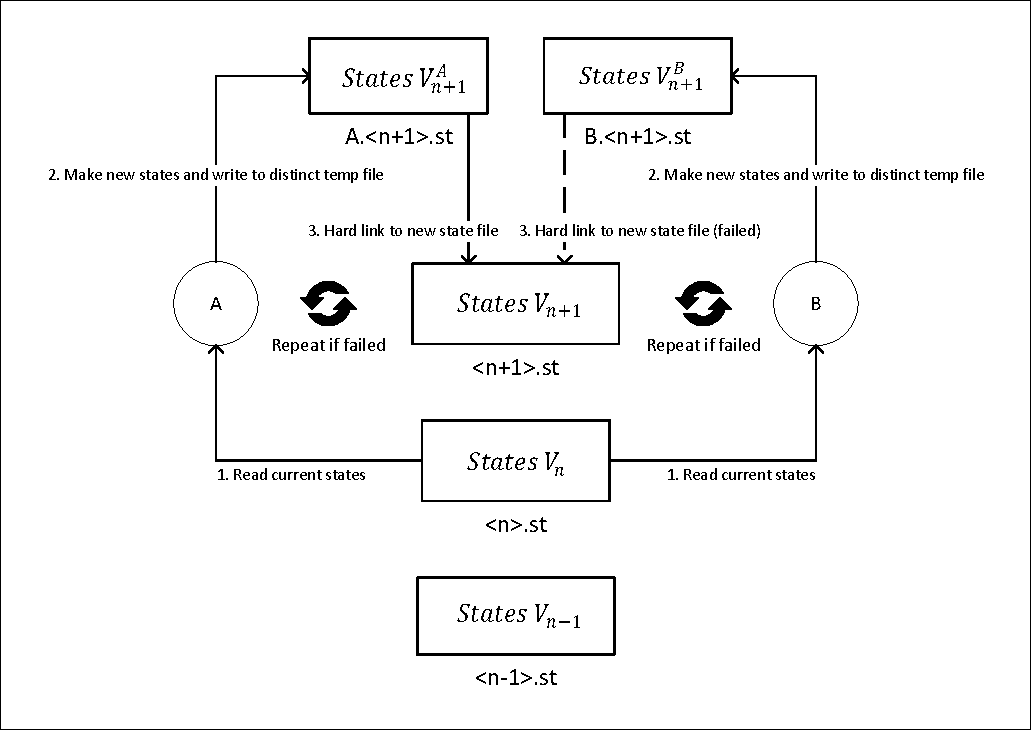
\includegraphics[width=1\textwidth, angle=0]{share-witness-implementation.pdf}
    \caption{Implement witness as a share}
    \label{fig:share-witness-implementation}
\end{figure}

In addition to share, the witness functionality can also be incorporated into cloud storage, such as Azure Storage or AWS S3. Many cloud storage vendors provide optimistic concurrency mechanism for updating object data. For instance, Azure Blob Storage allows clients to update a blob object using the original ETag, combined with a conditional header, to ensure that updates only occur if the ETag remains unchanged. This guarantees that no other client has updated the blob object concurrently. The infrequent access requirements and trivial payload size for witness make cloud storage an ideal solution for this function. Consequently, it provides a broader range of implementation options for end-users.



\subsection{Compatibility}\label{subsection:compatibility}
In a cluster without witness, the extended Raft algorithm functions identically to the Raft algorithm. This compatibility allows for an existing cluster based on the Raft algorithm to upgrade seamlessly to the extended Raft algorithm in a practical application. A binary upgrade can be applied to the current cluster to adopt the extended Raft algorithm. Subsequently, the upgraded cluster behaves just like a typical Raft-based cluster and does not include a witness.

Once all servers have been upgraded to accommodate the extended Raft algorithm, a membership reconfiguration operation can be conducted to add a witness into the cluster. Conversely, a cluster operating with the extended Raft algorithm can revert to the standard Raft algorithm through a binary downgrade after the removal of the witness from the cluster.

This flexibility is crucial for real-world applications because it negates the need to set up a new cluster and migrate data from the existing cluster to leverage the benefits of having a witness. Consequently, this minimizes disruptions and enhances the operational efficiency of these applications.